% --------------------------------------------------------------
% This is all preamble stuff that you don't have to worry about.
% Head down to where it says "Start here"
% --------------------------------------------------------------
 
\documentclass[12pt]{article}

\usepackage[margin=1in]{geometry} 
\usepackage{amsmath,amsthm,amssymb}
\usepackage[margin=1in]{geometry} 
\usepackage{amsmath,amsthm,amssymb}
%\usepackage[spanish]{babel} %Castellanización
\usepackage[T1]{fontenc} %escribe lo del teclado
\usepackage{inputenc} %Reconoce algunos símbolos
\usepackage{lmodern} %optimiza algunas fuentes
\usepackage{graphicx}
\graphicspath{ {images/} }
\usepackage{hyperref} % Uso de links

% To Display Chinese words
\usepackage{xeCJK}
% To Display Code
% \usepackage{listings}
\usepackage{minted}
% To Display csv file
\usepackage{csvsimple}
\usepackage{longtable}
\usepackage{booktabs}
% To Display hyperlink
\usepackage{hyperref}
 
\newcommand{\N}{\mathbb{N}}
\newcommand{\Z}{\mathbb{Z}}
 
\newenvironment{theorem}[2][Theorem]{\begin{trivlist}
\item[\hskip \labelsep {\bfseries #1}\hskip \labelsep {\bfseries #2.}]}{\end{trivlist}}
\newenvironment{lemma}[2][Lemma]{\begin{trivlist}
\item[\hskip \labelsep {\bfseries #1}\hskip \labelsep {\bfseries #2.}]}{\end{trivlist}}
\newenvironment{exercise}[2][Exercise]{\begin{trivlist}
\item[\hskip \labelsep {\bfseries #1}\hskip \labelsep {\bfseries #2.}]}{\end{trivlist}}
\newenvironment{problem}[2][Problem]{\begin{trivlist}
\item[\hskip \labelsep {\bfseries #1}\hskip \labelsep {\bfseries #2.}]}{\end{trivlist}}
\newenvironment{question}[2][Question]{\begin{trivlist}
\item[\hskip \labelsep {\bfseries #1}\hskip \labelsep {\bfseries #2.}]}{\end{trivlist}}
\newenvironment{corollary}[2][Corollary]{\begin{trivlist}
\item[\hskip \labelsep {\bfseries #1}\hskip \labelsep {\bfseries #2.}]}{\end{trivlist}}

\newenvironment{solution}{\begin{proof}[Solution]}{\end{proof}}

% write csv content in latex 
\begin{filecontents*}{test.csv}
ResNet18, ResNet18(pretrain), ResNet50, ResNet50(pretrain)
74.833, 81.082, 75.345, 81.423
\end{filecontents*}
 
\begin{document}
 
% --------------------------------------------------------------
%                         Start here
% --------------------------------------------------------------
 
\title{2019 Deep Learning and Practice \\ Lab 3 -- Diabetic Retinopathy Detection}
\author{0756110 李東霖}

\maketitle
\section{Introduction}

In this lab, I use ResNet to diagnose Diabetic Retinopathy. And also compare different between pretraining and no pretraining. There are some requirements in this lab as follows:

\begin{itemize}
\item Implement the ResNet18, ResNet50.
\item Implement the ResNet18, ResNet50 with loading pretraining parameters.
\item Compare and visualize the accuracy trend.
\item Implement custom DataLoader.
\item Calculate the confusion matrix
\end{itemize}


\subsection{Dataset}

Dataset has many images of retina and labels from diff diabetes state including no diabetes. Each image of size is 512x512x3 with RGB. 

\section{Experiment setup}

\subsection{My Dataloader}

Because shape of pytorch convolution layer need (N, C, H, W), I convert PIL image (512x512x3) to Tensor (3x512x512) by \verb|torchvision.transform.ToTensor|. In order to improve test accuracy and avoid overfitting, I use data augmentation in training data. But default setting is no data augmentation.
\par \ \par
\begin{minted}[frame=lines]{python}
class RetinopathyDataset(data.Dataset):
    def __init__(self, root, mode, augmentation=None):
        self.root = root
        self.img_name, self.label = getData(mode)
        self.mode = mode
        trans = []
        if augmentation:
            trans += augmentation
        trans += [transforms.ToTensor()]
        self.transforms = transforms.Compose(trans)
        print("> Found %d images..." % (len(self.img_name)))

    def __len__(self):
        return len(self.img_name)

    def __getitem__(self, index):
        path = os.path.join(self.root, self.img_name[index] + '.jpeg')
        img = PIL.Image.open(path)
        img = self.transforms(img)
        
        label = self.label[index]
        
        return img, label
\end{minted}
\par \ \par
I use random flip with horizontal and vertical to do data augmentation.

\begin{minted}[frame=lines]{python}
train_dataset = RetinopathyDataset('./data', 'train')
test_dataset = RetinopathyDataset('./data', 'test')

augmentation = [
    transforms.RandomHorizontalFlip(p=0.5),
    transforms.RandomVerticalFlip(p=0.5),
]
train_dataset_with_augementation = RetinopathyDataset('./data', 'train', augmentation=augmentation)
\end{minted}

And then use \verb|torch.utils.data.DataLoader| to convert dataset to dataloader.

\subsection{ResNet in my implementation}

ResNet is call "Deep residual network". What does mean "residual" ? We know weight layers of NN just like function : \( y = f(x) \). If we add inpux \( x \) to output; Like this : \( y = f(x) + x  \Rightarrow y - x = f(x) \). We let weight layers of NN to learn "residual" between output and input. This architecture also solves vanishing gradient so we design more layer in NN. Implementation of it has two type, one is BasicBlock another is BottleneckBlock. 
\par \ \par
Reference from \href{https://pytorch.org/docs/0.4.0/_modules/torchvision/models/resnet.html}{torchvision.models.resnet}. But I redesign it with variable kernel size.
\begin{minted}[frame=lines, breaklines]{python}
class BasicBlock(nn.Module):
    '''
    x = (in, H, W) -> conv2d -> (out, H, W) -> conv2d -> (out, H, W) + x
    '''
    expansion = 1
    
    def __init__(self, in_channels, out_channels, stride=1, kernel_size=3, downsample=None):
        super(BasicBlock, self).__init__()
        padding = int(kernel_size/2)
        self.activation = nn.ReLU(inplace=True)
        self.block = nn.Sequential(
            nn.Conv2d(
                in_channels, out_channels, 
                kernel_size=kernel_size, padding=padding, stride=stride, bias=False
            ),
            nn.BatchNorm2d(out_channels),
            self.activation,
            nn.Conv2d(
                out_channels, out_channels, 
                kernel_size=kernel_size, padding=padding, bias=False
            ),
            nn.BatchNorm2d(out_channels),
        )
        self.downsample = downsample
        
    def forward(self, x):
        residual = x
        out = self.block(x)
        
        if self.downsample is not None:
            residual = self.downsample(x)
        
        out += residual
        out = self.activation(out)
        
        return out

class BottleneckBlock(nn.Module):
    '''
    x = (in, H, W) -> conv2d(1x1) -> conv2d -> (out, H, W) -> conv2d(1x1) -> (out*4, H, W) + x 
    '''
    expansion = 4
    
    def __init__(self, in_channels, out_channels, stride=1, kernel_size=3, downsample=None):
        super(BottleneckBlock, self).__init__()
        padding = int(kernel_size/2)
        self.activation = nn.ReLU(inplace=True)
        self.block = nn.Sequential(
            nn.Conv2d(in_channels, out_channels, kernel_size=1, bias=False),
            nn.BatchNorm2d(out_channels),
            self.activation,
            nn.Conv2d(
                out_channels, out_channels,
                kernel_size=kernel_size, stride=stride, padding=padding, bias=False
            ),
            nn.BatchNorm2d(out_channels),
            self.activation,
            nn.Conv2d(out_channels, out_channels * self.expansion, kernel_size=1, bias=False),
            nn.BatchNorm2d(out_channels * self.expansion),
        )
        self.downsample = downsample
    
    def forward(self, x):
        residual = x
        out = self.block(x)
        
        if self.downsample is not None:
            residual = self.downsample(x)
        
        out += residual
        out = self.activation(out)
        
        return out
\end{minted}
\par \ \par
And then I also reference from  \href{https://pytorch.org/docs/0.4.0/_modules/torchvision/models/resnet.html}{torchvision.models.resnet} to redesign with variable structure of layer and number of channel.

\begin{minted}[frame=lines, breaklines]{python}
class ResNet(nn.Module):
    def __init__(self, block, layers, num_classes, start_in_channels=64):
        super(ResNet, self).__init__()
        
        self.current_in_channels = start_in_channels
        
        self.first = nn.Sequential(
            nn.Conv2d(
                3, self.current_in_channels,
                kernel_size=7, stride=2, padding=3, bias=False
            ),
            nn.BatchNorm2d(self.current_in_channels),
            nn.ReLU(inplace=True),
            nn.MaxPool2d(kernel_size=3, stride=2, padding=1),
        )
        
        self.layers = layers
        channels = self.current_in_channels
        for i, l in enumerate(layers):
            setattr(self, 'layer'+str(i+1), 
                    self._make_layer(block, channels, l, stride=(2 if i!=0 else 1) ))
            channels*=2
        
        self.avgpool = nn.AdaptiveAvgPool2d(1)
        self.fc = nn.Linear(self.current_in_channels, num_classes)
            
    def _make_layer(self, block, in_channels, blocks, stride=1):
        downsample=None
        if stride != 1 or self.current_in_channels != in_channels * block.expansion:
            downsample = nn.Sequential(
                nn.Conv2d(
                    self.current_in_channels, in_channels * block.expansion,
                    kernel_size = 1, stride=stride, bias=False
                ),
                nn.BatchNorm2d(in_channels * block.expansion)
            )
        
        layers = []
        layers.append(block(self.current_in_channels, in_channels, stride=stride, downsample=downsample))
        self.current_in_channels = in_channels * block.expansion
        for i in range(1, blocks):
            layers.append(block(self.current_in_channels, in_channels))
        
        return nn.Sequential(*layers)
    
    def forward(self, x):
        x = self.first(x)
        for i in range(len(self.layers)):
            x = getattr(self, 'layer'+str(i+1))(x)
        x = self.avgpool(x)
        # flatten
        x = x.view(x.size(0), -1)
        x = self.fc(x)
        
        return x
\end{minted}

Finally, I implement all basic compoments for ResNet. I use them to build ResNet18 and ResNet50 and also use \verb|torchvision| to make pretraining version. But architecture of pretrain model is different from my implementation, I need to separate them.

\begin{minted}[frame=lines]{python}
def ResNet18(pre_train=False):
    if pre_train:
        return PretrainResNet(num_classes=5, num_layers=18)
    return ResNet(BasicBlock, layers=[2,2,2,2], num_classes=5)
def ResNet50(pre_train=False):
    if pre_train:
        return PretrainResNet(num_classes=5, num_layers=50)
    return ResNet(BottleneckBlock, layers=[3,4,6,3], num_classes=5)
\end{minted}

\subsection{Evaluate through confusion matrix}

\begin{figure}[H]
\centering
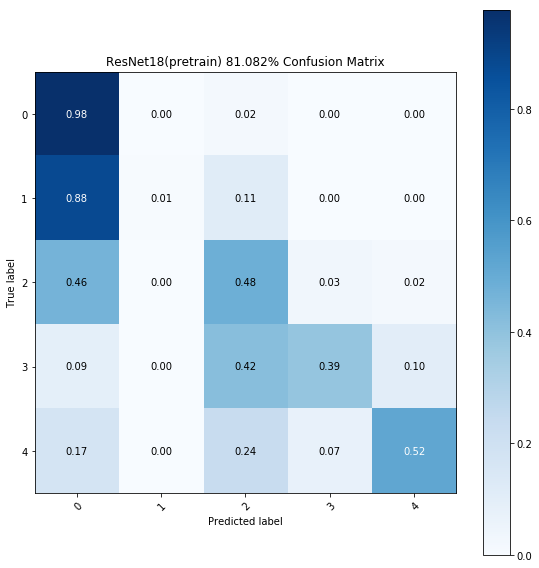
\includegraphics[width=\linewidth]{Images/ResNet18CM.png}
\caption{ResNet18 Confusion Matrix}
\end{figure}

\begin{figure}[H]
\centering
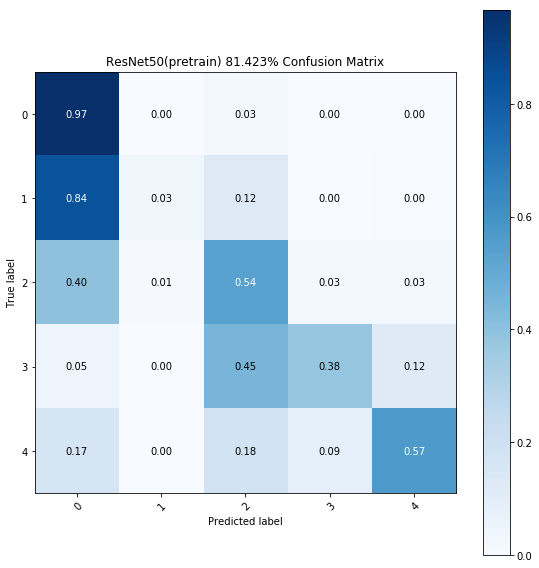
\includegraphics[width=\linewidth]{Images/ResNet50CM.png}
\caption{ResNet50 Confusion Matrix}
\end{figure}

This confusion matrix shows accuracy of class0 is good. But my model predict so many class1 to class0. Also predict output only have seldom class1. It maybe means no strong features exist in retina to classify class0 and class1. 

\section{Experimental results}

\subsection{The highest test accuracy}

\par
\begin{table}[H]
    \centering
    \csvautobooktabular{test.csv}
    \caption{Test accuracy}
    \label{tab:my_label}
\end{table}

\subsection{Comparison figures}

I draw two dash lines to mark 75\% and 82\%.

\begin{figure}[H]
\centering
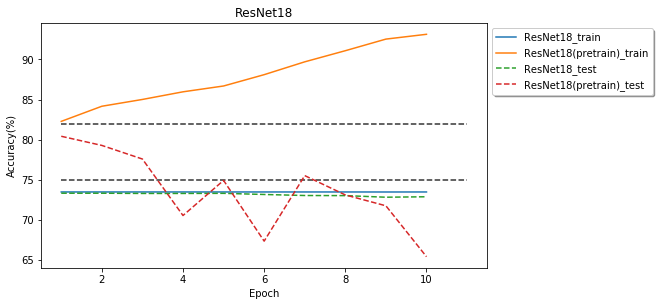
\includegraphics[width=\linewidth]{Images/ResNet18.png}
\caption{ResNet18}
\end{figure}

\begin{figure}[H]
\centering
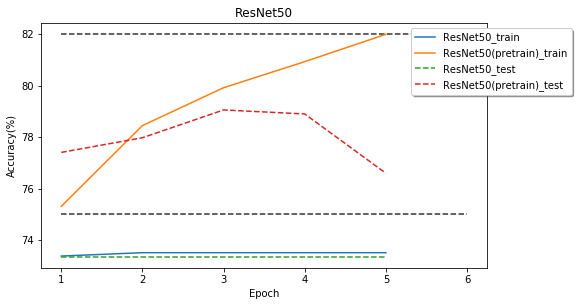
\includegraphics[width=\linewidth]{Images/ResNet50.png} 
\caption{ResNet50}
\end{figure}

I find model without pretrain can't increase accuracy. Model with pretrain even grow up accuracy in training but it fail in testing. Specially, model with pretrain will decrease test accuracy. That means model with pretrain occur overfitting.

\section{Discussion}

\subsection{Data augmentation}

In order to prevent overfitting, I tried to add some data augmentation in training data.

\begin{figure}[H]
\centering
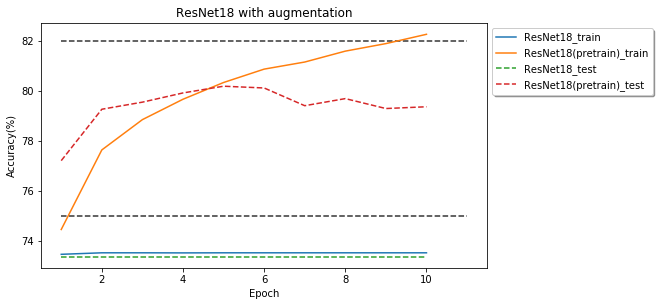
\includegraphics[width=\linewidth]{Images/ResNet18withDA.png}
\caption{ResNet18 with data augmentation}
\end{figure}

\begin{figure}[H]
\centering
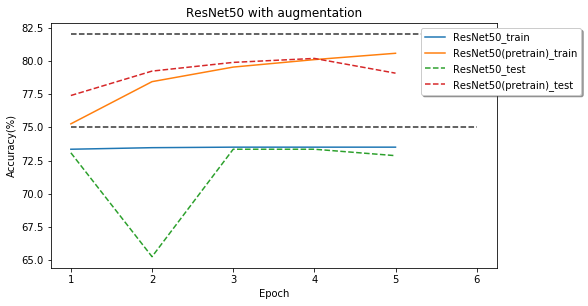
\includegraphics[width=\linewidth]{Images/ResNet50withDA.png}
\caption{ResNet50 with data augmentation}
\end{figure}

\subsection{More epoch and batch to train model without pretrain}

To make model(without pretrain) trainable, I set epoch size and batch size more than before. Finally, I saw the accuracy growth. But I also saw the overfitting in model with pretrain. I think some features only exist in testing dataset.

\begin{figure}[H]
\centering
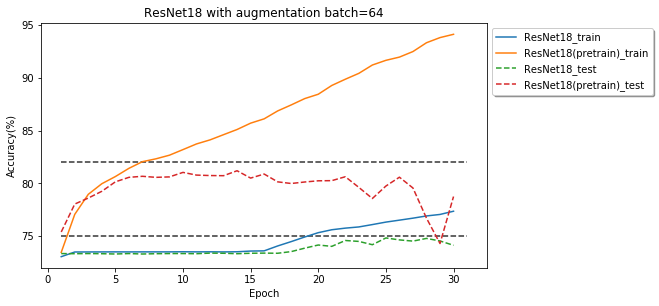
\includegraphics[width=\linewidth]{Images/ResNet18withLE.png}
\caption{ResNet50 with more epoch and batch}
\end{figure}

\begin{figure}[H]
\centering
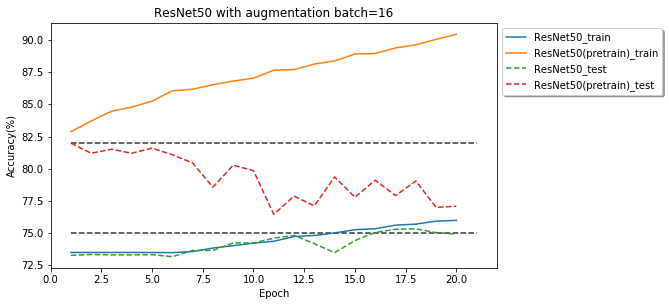
\includegraphics[width=\linewidth]{Images/ResNet50withLE.png}
\caption{ResNet50 with more epoch and batch}
\end{figure}

% --------------------------------------------------------------
%     You don't have to mess with anything below this line.
% --------------------------------------------------------------
 
\end{document}